\question 下图所示的曼彻斯特编码表示的比特串为( ~)。~

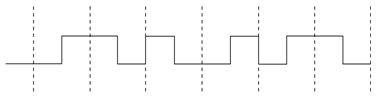
\includegraphics[width=1.04167in,height=1.04167in]{computerassets/60B84D760E1212C1E488F5431E53DC46.png}
\par\twoch{\textcolor{red}{011001}}{100110}{111110}{011110}
\begin{solution}曼彻斯特编码每一周期分为两个相等的间隔。二进制``1''在发送时,在第一个间隔中为高电压,在第二个间隔中为低电压;二进制``0''正好相反,首先是低电压,然后是高电压。根据所给图形可知,该曼彻斯特编码表示的比特串为011001。
~ ~
~提醒:有些教材或者辅导书恰好和本题的``1''和``0''的表现形式相反,这个不用疑惑,知道即可,考研不可能考这种题,仅仅作为练习用以了解曼彻斯特编码。
\end{solution}
\question 有一个调制解调器,它的调制星形图如下图所示。当它传输的波特率达到2400Baud时,实际传输的比特率为(
~)。

~
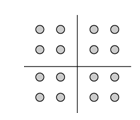
\includegraphics[width=1.04167in,height=1.04167in]{computerassets/B4EF6AF3A7F2C9C0FE3B7D8F48920A13.png}
\par\fourch{2400bit/s}{4800bit/s}{\textcolor{red}{9600bit/s}}{19200bit/s}
\begin{solution}如题干图所示,对于该调制解调器的每个变化能够表示16种不同的信号。所以每个变化可以表示的比特数为n=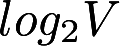
\includegraphics[width=0.43750in,height=0.14583in]{texmath/59cdc05Cdpi7B3507Dlog_2V},解得n=4,比特率=波特率×n,即9600bit/s。
\end{solution}
\question 若图2-16为10 Base-T网卡接收到的信号波形,则该网卡收到的比特串是( ~)。
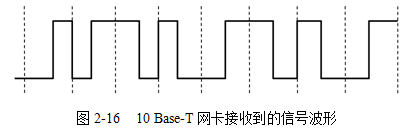
\includegraphics[width=3.33333in,height=1.07292in]{computerassets/3FAE39CB101AFF3BB8DBABF6F9D0CF6B.png}
\par\fourch{\textcolor{red}{0011 0110}}{1010 1101}{0101 0010}{1100 0101}
\begin{solution}10
Base-T代表的就是传统的以太网,而以太网使用的是曼彻斯特编码,而该编码将每个码元分成两个相等的间隔。前面一个间隔为高电平而后一个间隔为低电平表示码元1;码元0正好相反。于是可以得到该网卡收到的比特串是0011
0110。
\end{solution}
\question 下列有关曼彻斯特编码的说法,正确的是( )。
\ding{192}.每个信号起始边界作为时钟信号有利于同步
\ding{193}.将时钟与数据取值都包含在信号中
\ding{194}.这种模拟信号的编码机制特别适合传输声音
\par\twoch{仅\ding{192}、\ding{193}}{仅\ding{193}、\ding{194}}{仅\ding{194}}{\textcolor{red}{仅\ding{193}}}
\begin{solution}\ding{192}:曼彻斯特编码使用每个码元的中间跳变来作为同步时钟,并不是起始边界,故\ding{192}错误。
\ding{193}:曼彻斯特编码是将时钟和数据包含在数据流中,在传输代码信息的同时,也将时钟同步信号一起传输到对方,故\ding{193}正确。
\ding{194}:曼彻斯特编码是数字信号的编码机制,不适合用来传输声音,故\ding{194}错误。
注:曼彻斯特编码与差分曼彻斯特编码都属于自含时钟编码方式。曼彻斯特编码常用于局域网。
\end{solution}
\question 下列说法错误的是( )。 \ding{192}.差分曼彻斯特编码不可进行差错控制
\ding{193}.曼彻斯特编码所占用的频带宽度是非归零码的两倍
\ding{194}.曼彻斯特编码每位的中间不跳变表示信号的取值为0
\par\twoch{仅\ding{192}、\ding{193}}{仅\ding{193}、\ding{194}}{\ding{192}、\ding{193}和\ding{194}}{\textcolor{red}{仅\ding{194}}}
\begin{solution}\ding{192}:差分曼彻斯特编码是属于物理层的编码,肯定不能进行差错控制,故\ding{192}正确。
\ding{193}:曼彻斯特编码由于信号中不但包含数据,而且还包含同步时钟(各占一半),而非归零码全部都是数据,因此曼彻斯特编码所占用的频带宽度是非归零码的两倍,故\ding{193}正确。
\ding{194}:曼彻斯特编码用电压的跳变来区分码元1与码元0,故每位中间都有跳变,故\ding{194}错误。
\end{solution}
\question 脉冲编码调制(PCM)的过程是( )
\par\twoch{\textcolor{red}{采样、量化、编码}}{采样、编码、量化}{量化、采样、编码}{编码、量化、采样}
\begin{solution}脉冲编码调制主要经过3个过程:采样、量化和编码。采样过程将连续时间模拟信号变为离散时间、连续幅度的抽样信号;量化过程将抽样信号变为离散时间、离散幅度的数字信号;编码过程将量化后的信号编码为一个二进制码组输出。此知识点属于死记硬背型的,无需了解其原理。
\end{solution}
